This chapter covers the detection of rectangular structured regions.

An abstract discussion of various properties of algorithms is presented, and the desirable traits brought forth by each.
Then, a selection of concrete algorithms are described, and their merits and weaknesses examined.


\section{Key concepts}
An \emph{absolute structured position} refers to the position of a structured element with respect to the boundaries of its structured region.
A \emph{relative structured position} refers to the position of a structured element with respect to other structured elements within its structured region. Figure~\ref{fig:structured-position} shows this through an example.


%% Relative vs absolute
\begin{figure}
\newcommand{\nodesize}{1.2}
\newcommand{\rows}{4}
\newcommand{\cols}{4}
\newcommand{\rowsize}{\rows*\nodesize}
\newcommand{\colsize}{\cols*\nodesize+2*0.1}

% Node at position r, c, label
\newcommand{\nodeat}[3]{
	\pgfmathsetmacro{\lerow}{ (\rows - #1) * \nodesize - (\nodesize / 2) - 0.1}
	\pgfmathsetmacro{\lecol}{ (#2 * \nodesize) + (\nodesize / 2) + 0.1}
	\node at (\lecol, \lerow) {#3}
}

\sidebyside
{
	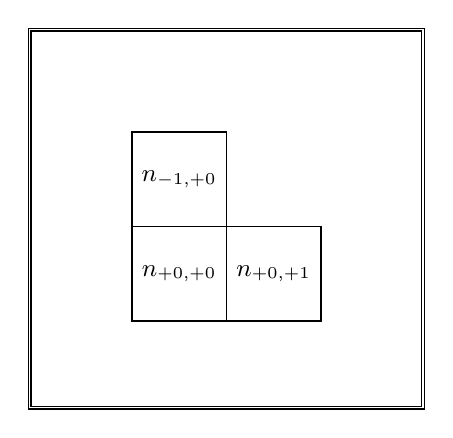
\begin{tikzpicture}
		\tikzstyle{every node}=[draw, shape=rectangle, minimum size=\nodesize cm, font=\small];
		\draw[double] (0,0) rectangle (\colsize,\rowsize);
		\nodeat{2}{1} {$n_{+0,+0}$};
		\nodeat{1}{1} {$n_{-1,+0}$};
		\nodeat{2}{2} {$n_{+0,+1}$};
	\end{tikzpicture}
	\caption{Relative structured position\label{fig:relative-structured-position}}
}
{
	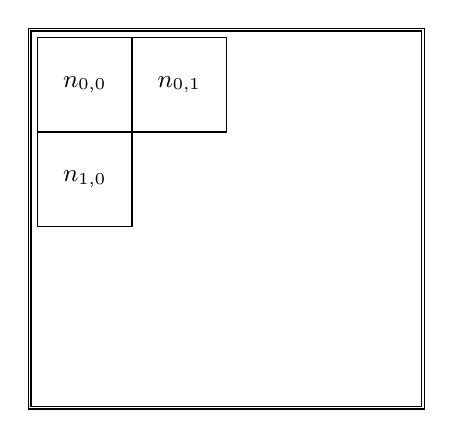
\begin{tikzpicture}
		\tikzstyle{every node}=[draw, shape=rectangle, minimum size=\nodesize cm, font=\small];
		\draw[double] (0,0) rectangle (\colsize,\rowsize);
		\nodeat{0}{0} {$n_{0,0}$};
		\nodeat{1}{0} {$n_{1,0}$};
		\nodeat{0}{1} {$n_{0,1}$};
	\end{tikzpicture}
	\caption{Absolute structured position\label{fig:absolute-structured-position}}
}
\caption{Depiction of \emph{relative} structured position versus \emph{absolute} structured position. The row and column counts are increasing down and to the right, respectively. The borders indicate structured regions, whose origin resides in the top-left corner.\label{fig:structured-position}}
\end{figure}



\section{Properties of detection algorithm}

\subsection{Eager detection}
An eager (or greedy) detection algorithm will include every structured element if finds immediately, regardless of the long term consequences. While this strategy may lead to suboptimal results, it avoids backtracking the structure detection which may be prohibitively costly. Figure~\ref{fig:eager-detection} depicts the sub-optimality of eager detection in contrast with non-eager detection.


\begin{figure}
\pgfplotstableread{
	2 2 2 2 2 2 0
	2 2 1 2 2 0 0
	0 0 1 0 0 0 0
	0 0 1 0 0 0 0
}{\eagermatrix}
\pgfplotstableread{
	2 2 2 2 2 2 0
	2 2 0 2 2 0 0
	1 1 1 1 1 1 1
	1 1 1 1 1 1 1
}{\noneagermatrix}

\sidebyside
{
	\drawmatrix[cell wd=0.6, cell ht=0.6]{\eagermatrix}
	\caption{Eager detection may greedily add the northern cell, yielding a suboptimal structured region.}
}
{
	\drawmatrix[cell wd=0.6, cell ht=0.6]{\noneagermatrix}
	\caption{A non-eager algorithm could instead decide to ignore the northern cell, yielding a larger structured region.}
}
\caption{Eager versus non-eager detection. The dotted region represents unstructured elements. Blue cells denote structured elements detected as forming a rectangular structured region; white cells denote the remaining structured elements.\label{fig:eager-detection}}
\end{figure}



\subsection{Contiguous detection}
\label{subsec:contiguous-detection}
An algorithm which exhibits continuous detection always adds a structured element which is contiguous to the structured region thus far. The implication is that the relative structured position is always known. This greatly simplifies detection, as all adjacent structured elements are known at any point in time, and structured elements need not be repositioned in the structured region. Figure~\ref{fig:contiguous-detection} contrasts contiguous detection with non-contiguous detection.

In the case of non-contiguous detection, any non-contiguous blobs need to be consolidated. These blobs may be one of three cases:
\begin{enumerate}
\item Disjoint
These may simply be taken as two separate structured regions.

\item Compatible
The blobs can be merged in a lossless manner to form a single structured region.

\item Incompatible
The blobs cannot be merged without loss of structure due to inconsistencies between the blobs. It is then necessary to discard some structured elements.
\end{enumerate}

Examples of the three cases are shown in figure~\ref{fig:non-contiguous-detection}.


% Contiguous versus non-contiguous
\begin{figure}
\pgfplotstableread{
	0 1 1 1 0 0 0 0 0
	0 1 1 1 1 0 0 0 0
	0 1 1 1 0 0 0 0 0
	0 0 1 0 0 0 0 0 0
	0 0 0 0 0 0 0 0 0
}{\contiguousmatrix}
\pgfplotstableread{
	0 1 1 1 0 0 0 0 0
	0 1 1 1 1 0 0 1 0
	0 1 1 1 0 0 1 1 0
	0 0 1 0 0 0 0 0 0
	0 0 0 0 0 0 0 0 0
}{\noncontiguousmatrix}

\sidebyside
{
	\drawmatrix[cell wd=0.6, cell ht=0.6]{\contiguousmatrix}
	\caption{Contiguous detection always adds cells adjacent to the structured region detected thus far.}
}
{
	\drawmatrix[cell wd=0.6, cell ht=0.6]{\noncontiguousmatrix}
	\caption{Non-contiguous detection may add cells which do not border the structured region detected thus far.}
}
\caption{Contiguous detection versus non-contiguous detection algorithms. White cells denote structured elements which have not been added to the structured region. Blue cells denote structured elements detected thus far.\label{fig:contiguous-detection}}
\end{figure}

% Types of non-contiguous
\begin{figure}
\sidebysidethreeverticaltop
{
	\includesvg[svgpath=images/detection-algorithms/,width=\imagewidth]{disjoint-blobs}
	\caption{Disjoint blobs of structured elements.}
}
{
	\includesvg[svgpath=images/detection-algorithms/,width=\imagewidth]{compatible-blobs}
	\caption{Compatible blobs of structured elements.}
}
{
	\includesvg[svgpath=images/detection-algorithms/,width=\imagewidth]{incompatible-blobs}
	\caption{Incompatible blobs of structured elements. The two dashed cells are not adjacent in the mesh, but if added as structured element they would have adjacent positions in the structured region.}
}
\caption{Cases that may arise with non-contiguous detection.\label{fig:non-contiguous-detection}}
\end{figure}


\subsection{Post processing requirements}
Different algorithms will require different levels of post-processing in order to yield a rectangular structured region. Some may require a simple operation, such as trimming incomplete rows, while others may require more complex operations to achieve this goal.


\subsection{Detection traversal patterns}
The order in which structured elements are detected in a structured region is important; it imposes some constraints on the data structure representing it. Given the dimensions of the structured region, and knowledge of the absolute structured positions of elements as they are discovered, a simple 2D array allocation would suffice. Any detection order, as is convenient, may be used in this case. However, neither of those facts are known a priori in general.

Various detection traversals orders and their merits are discussed below. Figure~\ref{fig:detection-traversal-patterns} outlines some examples.

\subsubsection{Single-row append-only}
\label{append-detection}
The structured region is grown in a constant direction, for example a single row of structured elements, appended to consecutively. This can be implemented efficiently using either a singly-linked list or a dynamic array with amortized constant time append operation.

\subsubsection{Single-row append/prepend}
\label{append-prepend-detection}
The structured region is grown in either of two directions, for example a single row of structured elements, appended and prepended to. This can be implemented efficiently using a double-ended queue with amortized constant time append and prepend operations.

\subsubsection{Row-oriented detection}
The structured region is represented as a group of rows, with the elements in individual rows grown using one of the above methods. The order in which the rows themselves are grown may also be utilize the same methods, with a nested data structure being a suitable implementation. For example, if rows are detected in an append-only fashion, and the individual elements are detected using append and prepend operations, then a suitable data structure would be a singly-linked list of double-ended queues.

\subsubsection{Indeterminate order detection}
The structured region is grown in a non-linear order: grown elements may not always be contiguous to the structured region thus far. If the growth is indeed non-contiguous, the relative structured positions are \emph{not} always known, and structured elements may need to be repositioned. A possible implementation would be a jagged 2D array, that is an array of arrays, which is expanded as needed. A flat-array-based 2D array would (in the worst case) require reallocating all elements upon expansion, as opposed to reallocating a single row in the case of a jagged 2D array.

Assuming contiguous structure detection, then when adding a new structured element $e_{new}$ the following holds:
\begin{enumerate*}[label=\alph*)]
\item we know exactly which existing structured elements must be adjacent to $e_{new}$, and
\item we only need to check the adjacency between $e_{new}$ and existing structured elements.
\end{enumerate*}
On the other hand if structure detection is non-contiguous, then we may later discover that some structured elements are no longer mutually compatible. We thus must check the adjacency between existing structured elements as we add new ones. Figure~\ref{fig:contiguous-comparison}


\begin{figure}
\pgfplotstableread{
	1 1 1 2 0
	1 1 1 2 0
	1 1 6 2 0
	1 5 9 0 0
	1 1 0 0 0
}{\contiguousmatrix}
\pgfplotstableread{
	1 1 1 2 1
	1 1 1 2 1
	1 1 6 2 1
	1 5 9 7 1
	1 1 0 0 0
}{\noncontiguousmatrix}

\sidebysidevertical
{
\drawmatrix[cell wd=0.8, cell ht=0.8]{\contiguousmatrix}
\caption{Contiguous detection, with $\times$ denoting the currently considered element. We must check that $\times$ is adjacent to both $A$ and $B$, but is not adjacent to any other structured element detected thus far.}
\label{subfig:contiguous}
}
{
\drawmatrix[cell wd=0.8, cell ht=0.8]{\noncontiguousmatrix}
\caption{Non-contiguous detection, with $\times$ denoting the currently considered element, which if added will join two disjoint components. We must check that $\times$ is adjacent to $A$, $B$, and $C$, but not adjacent to any other existing structured element. Furthermore, we must check that the existing structured elements in one component are \emph{not} adjacent to any structured elements in the other component, except through $\times$.}
\label{subfig:non-contiguous}
}

\caption{Comparing the costs of contiguous structure detection~\ref{subfig:contiguous} and non-contiguous structure detection~\ref{subfig:non-contiguous}.}
\label{fig:contiguous-comparison}
\end{figure}


% Detection traversal patterns
\begin{figure}
\begin{subfigure}[t]{0.45\textwidth}
	\centering
	\includesvg[svgpath=images/detection-algorithms/,width=\textwidth]{append-detection}
	\caption{Single-row append detection.}
\end{subfigure}
\begin{subfigure}[t]{0.45\textwidth}
	\centering
	\includesvg[svgpath=images/detection-algorithms/,width=\textwidth]{append-prepend-detection}
	\caption{Single-row append/prepend detection.}
\end{subfigure}
\begin{subfigure}[b]{0.45\textwidth}
	\centering
	\includesvg[svgpath=images/detection-algorithms/,width=0.8\textwidth]{row-oriented}
	\vspace{4.5mm}
	\caption{Row-oriented detection, with rows detected in an append-only fashion, and elements within rows in an append/prepend fashion.}
\end{subfigure}
\begin{subfigure}[b]{0.45\textwidth}
% \vfill
	\centering
	\includesvg[svgpath=images/detection-algorithms/,width=\textwidth]{indeterminate-detection}
	\caption{Indeterminate order detection. Note that some possible regions of expansions are not adjacent to the presently detected structured region.}
\end{subfigure}

\caption{Examples of detection traversal patterns. The blue blocks represent presently detected structured regions. The dashed pink blocks represent possible regions for expansion.\label{fig:detection-traversal-patterns}}
\end{figure}



\section{Detection algorithms}

\subsection{Length-first search}

\begin{enumerate}
\item Starting from a seed vertex, grow a quad.

\item The quad is grown along one axis, both forwards and backwards, as far as possible, forming the length of the structured region. This is a per-row append/prepend traversal.
\item The row grown above is extended along the orthogonal axis, both forwards and backwards, as far as possible. Each expanded row must have the length of the initial row exactly, forming the width of the structure region. This is a row-oriented append/prepend traversal.
\end{enumerate}

The detection is clearly contiguous, with all structured element insertions running in amortized constant time. Only a constant amount of extra storage is required.

The algorithm is also an eager one, deciding the length of the structured region based on the first row it detects. This simple approach, however, can result in suboptimal detection.



\subsection{Descending-staircase search}
\begin{enumerate}
\item Follow the same steps as in length-first search, with one exception: in step~\ref{step:row-expansion}, each expanded row may have a length which is at most the length of its predecessor.
\item Find the rectangle with the maximum area, using an algorithm such as XXXXXX.
\end{enumerate}



Two types of techniques exist: seed-based, and global based. A seed-based technique starts with a seed, and grows from there. A global-based technique starts with all the orthogonal axis